\PassOptionsToPackage{type=CC,modifier=by,version=4.0}{doclicense}
\documentclass[conference,a4paper]{cs-techrep}
\pdfoutput=1 % pdflatex hint for arxiv.org (within first 5 lines)

% Class cs-techrep.cls loads biblatex / biber with predefined options
\addbibresource{embedded.bib}       % its content is declared below, embedded within this tex-file
\addbibresource{webdev_commons.bib} % includes REST, React, Angular, Vue, Svelte, Docker, AWS-*, Socket.IO, and many more!
\addbibresource{cpn_all_all.bib}    % includes all previous CyberLytics@OTH-AW technical reports

%% Workaround to make acronym working on current miktex version
%% https://tex.stackexchange.com/questions/735500/problem-with-amsmath-cleveref-acronym
%\makeatletter
%\AtBeginDocument
%{
%	\def\ltx@label#1{\cref@label{#1}}%add braces
%	\def\label@in@display@noarg#1{\cref@old@label@in@display{#1}}%remove braces
%	\def\label@in@mmeasure@noarg#1{%
%		\begingroup%
%		\measuring@false%
%		\cref@old@label@in@display{#1}%remove braces for multline, see https://tex.stackexchange.com/q/737204/2388
%		\endgroup}%  
%} %
%\makeatother
%% End Workaround


% ======================================================================
% EDIT THESE:

\cstechrepAuthorListTex{Dotzler Martin, Ehrles Andreas, Taach Eduard, Wegerer Nikolas,\\ Weinhut Justin, Christoph P.\ Neumann\,\orcidlink{0000-0002-5936-631X}}
\cstechrepAuthorListBib{Dotzler Martin \& Ehrles Andreas \& Taach Eduard \& Wegerer Nikolas \& Weinhut Justin \& Christoph P. Neumann}

% Capitalization: https://capitalizemytitle.com/style/Chicago/
\cstechrepTitleTex{GetraenkeIO: Eine Getränkelagerverwaltung mit Bestandsstatistik für Vereinsheime}
 % IF you need manual linebreaks in the titel, then clone the title without linebreaks for BibTeX:
\cstechrepTitleBib{{\cstechrepTitleTex}}

%\cstechrepDepartment{CyberLytics\-/Lab at the Department of Electrical Engineering, Media, and Computer Science}
\cstechrepDepartment{CyberLytics\-/Lab an der Fakultät Elektrotechnik, Medien und Informatik} % DE
\cstechrepInstitution{Ostbayerische Technische Hochschule Amberg\-/Weiden}
%\cstechrepAddress{Amberg, Germany}
\cstechrepAddress{Amberg, Deutschland} % DE
%\cstechrepType{Technical Report}
\cstechrepType{Technischer Bericht} % DE
\cstechrepYear{2025}
\cstechrepMonth{7}
\cstechrepNumber{CL-TR-\cstechrepYear{}-42}
%\cstechrepLang{english}  % en-US
\cstechrepLang{ngerman} % DE

% Special remark on babel/csquotes terminology in regard with US-vs-UK:
% en-US  = [english]/[american]/[usenglish] (+ [canadian])
% en-UK  =           [british] /[ukenglish] (+ [australian]) <OXFORD>
% For cs-techrep (like ACM), the recommended english variant is en-US!

% DO NOT DELETE THIS:
\filecontentsForceExpansion|[] % force command expansion inside a filecontents* environment
\begin{filecontents*}[overwrite]{selfref.bib}
    @TECHREPORT{selfref,
        author = {|cstechrepAuthorListBib},
        title  = {\cstechrepTitleBib},
        institution = {\cstechrepInstitution, \cstechrepDepartment},
        type   = {\cstechrepType},
        number = {\cstechrepNumber},
        year   = {|cstechrepYear},
        month  = {|cstechrepMonth},
        langid  = {|cstechrepLang},
    }
\end{filecontents*}

% ======================================================================
% EDIT THIS:

\begin{filecontents}[overwrite]{embedded.bib}
@Online{conatiners,
	author = {{IBM}},
	title = {Was sind Container?},
	url = {https://www.ibm.com/de-de/topics/containers},
	year = {2025}
}
@Online{sqlmodel,
	author = {Sebastián Ramírez},
	title = {SQLModel},
	url = {https://https://sqlmodel.tiangolo.com/},
	year= {2025}
}
@Online{openapi,
	author = {{The Linux Foundation}},
	title = {OpenAPI-Spezifikation},
	url = {https://spec.openapis.org/oas/latest.html},
	year= {2025}
}
@Online{swagger,
	author = {{SMARTBEAR}},
	title = {Swagger},
	url = {https://swagger.io/},
	year= {2025}
}

@online{ieee2015howto,
    author = {Michael Shell},
    title = {How to Use the {IEEEtran} \LaTeX\ Class},
    url = {http://mirrors.ctan.org/macros/latex/contrib/IEEEtran/IEEEtran_HOWTO.pdf},
    year = {2015}
}
@online{ieee2018formattingrules,
    author = {{IEEE}},
    title = {Conference Template and Formatting Specifications},
    url = {https://www.ieee.org/content/dam/ieee-org/ieee/web/org/conferences/Conference-template-A4.doc},
    year = {2018}
}
@online{iaria2014formattingrules,
    author = {{IARIA}},
    title = {Formatting Rules},
    url = {http://www.iaria.org/formatting.doc},
    year = {2014}
}
@online{iaria2009editorialrules,
    _author = {Cosmin Dini},
    author = {{IARIA}},
    title = {Editorial Rules},
    url = {https://www.iaria.org/editorialrules.html},
    year = {2009}
}
@online{languagetool,
    author = {{LanguageTooler GmbH}},
    title  = {{LangueTool}},
    url    = {https://languagetool.org/overleaf}
}
@online{overleaf,
    author = {{Digital Science UK Limited}},
    title  = {{Overleaf}},
    url    = {https://www.overleaf.com}
}
\end{filecontents}

\usepackage{fontawesome} % i.a., \faWarning{}
\usepackage{relsize}     % i.a., \textsmaller{...}
\usepackage{lipsum}      % for blindtext
\usepackage{enumitem}
% ======================================================================

% cf. https://ctan.org/pkg/acronym
% Usage:
% singular, within sentence       = \ac{gui}
% singular, beginning of sentence = \Ac{gui}
% plural, within sentence         = \acp{gui}
% plural, beginning of sentence   = \Acp{gui}
\begin{acronym}
    \acro{gui}[GUI]{Graphical User Interface}
    \acro{ide}[IDE]{Integrated Development Environment}
    \acro{orm}[ORM]{Object-Relational Mapping}
    \acro{cors}[CORS]{Cross-Origin Resource Sharing}
    \acro{crud}[CRUD]{Create, Read, Update und Delete}
\end{acronym}

% https://www.silbentrennung24.de/
% https://www.hyphenation24.com/
\hyphenation{block-chain block-chains Ethe-re-um}

\begin{document}
\selectlanguage{\cstechrepLang}

\maketitle

\begin{abstract}
\lipsum[1][3-10]
\{\,\faWarning{}The abstract does neither mention a teaching module nor a team/project,
it is a summary of the content, thus, the objectives and architecture.
Do NOT remove the abstract \faWarning{}, this section is mandatory.
You should consider comparing your self-written abstract with the result of a generative AI that summarizes your content after you have written a nearly stable draft version. However, do not use a verbatim copy to replace your abstract, just use generative AI for inspirational purposes.\}
\end{abstract}

% A list of IEEE Computer Society appoved keywords can be obtained at
% http://www.computer.org/mc/keywords/keywords.htm
\begin{IEEEkeywords}
D.2.0.c Software engineering for Internet projects, D.2.2.c Distributed/Internet based software
engineering tools and techniques
\end{IEEEkeywords}

\section{Einleitung und Projektziele}

The cs-techrep formatting is adopted both from \textsmaller{IEEE} \cite{ieee2018formattingrules} and \textsmaller{IARIA} \cite{iaria2014formattingrules} styles.
The cs-techrep \LaTeX\ class is based on \textsmaller{IEEE}tran class \cite{ieee2015howto}.
In addition, be aware of the supplementary \textsmaller{IARIA} editorial rules \cite{iaria2009editorialrules} \faWarning{} that provide a beginner-friendly set of further advices.
It is recommended to use a grammar tool, e.\,g., the LanguageTool \cite{languagetool} browser plugin in combination with Overleaf \cite{overleaf}.

The title of your paper should not exceed two lines \faWarning{}. In exceptional cases, three lines might be allowed. A four-line-title is absolutely forbidden (hint: use the longer form in the abstract).

For capitalization of titles and section headings, use a web tool like \href{https://capitalizemytitle.com/style/Chicago/}{Capitalize My Title} \faWarning{} with the option \texttt{Chicago} for capitalization rules by Chicago Manual of Style (CMOS).

The pipe symbol \textquote{\textbar{}} in the section headings represents alternatives! Choose one and remove the others \faWarning{}. The selectively provided quoted terms are special German alternatives. You may deviate from the structure of this example document and its exemplary section headings.

The problem statement needs to be written from perspective of a subject-matter expert (\textquote{Fachkonzept}). Like an elevator pitch / mission statement \faWarning{} and NOT from a technical perspective.

\section{Optional: Related Work \textbar{} State of the Art \textbar{} Methods \textbar{} Data Acquisition}
\lipsum[2]

\section{Architekturziele} % \textbar{} \textquote{Architekturziele}}
Provides
(1) a visualization of the external systems and users with which the system interacts (\textquote{Kontextabgrenzung}),
(2) the most important technical and organizational preconditions (\textquote{Rahmenbedingungen}),
(3) quality/non-functional requirements (\textquote{Qualitätsziele}), and/or
(4) architectural style design decisions with formative patterns of the solution (\textquote{Architekturstil})
as well as (5) the applied programming language(s).

\section{Architektur von GetraenkeIO} %of CatchyName \textbar{} Results \textbar{} Structural Design \textbar{} \textquote{Bausteinsicht}

\subsection{Technologie-Stack} % \textbar{} Overall System \textbar{} \textquote{Gesamtsystem}}
Die GetraenkeIO-Anwendung soll auf einer dreischichtigen Architektur, bestehend aus Frontend, Backend und Datenhaltungsschicht bestehen.
Jede Schicht soll von den anderen abgegrenzt auf einem eigenen Container \cite{conatiners} laufen.
Das Frontend besteht aus einer React-Anwendung \cite{react}.
Als Backend wird eine Python-Anwendung \cite{python} verwendet.
Diese benutzt das Web-Framework FastAPI \cite{fastapi} und stellt damit dem Frontend eine RESTful-Schnittstelle \cite{restful} zum Datenaustausch zur Verfügung.
Zur Datenhaltung wird die relationale Datenbank PostgreSQL \cite{postgresql} genutzt.
Die Kommunikation zwischen Datenbank und Backend übernimmt das Framework SQLModel \cite{sqlmodel}, welches Mittels \ac{orm} die Datenbanktabellen als Python-Objekte zur Verfügung stellt.

\begin{figure}
	\centering
	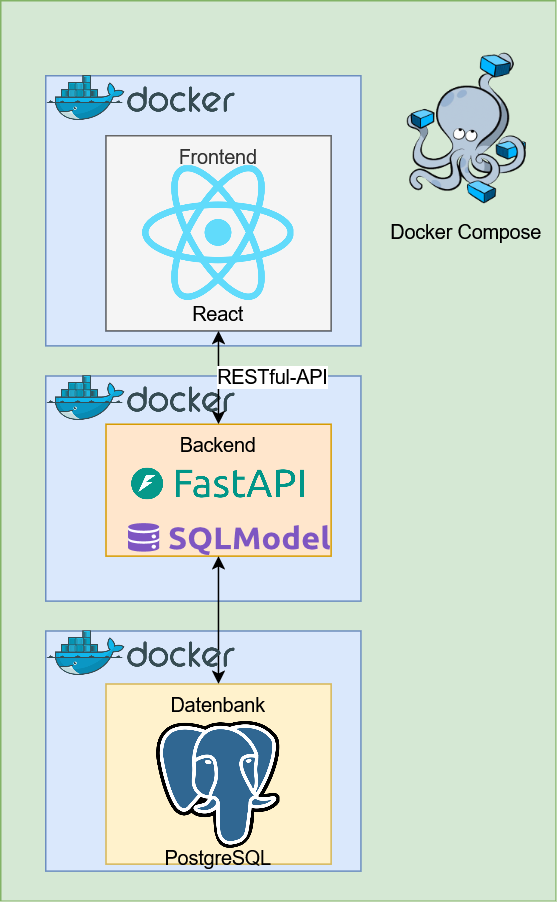
\includegraphics[width=0.9\linewidth]{Bausteinsicht-Architektur.drawio}
	\caption{Bausteinsicht über den Technologie-Stack und die verwendeten Technologien und deren Zusammenspiel.}
	\label{fig:bausteinsicht-architektur}
\end{figure}


\subsubsection{Vorlage Hr. Neumann}
Provides
(1) design decisions based on the previously defined requirements and
(2) a visualization of the functional structure at top level including relationships (\textquote{Grobe Zerlegung}), thus, gives an overview on modules, frameworks, and middleware.

In discussions of multi-tier architecture, layer is often used interchangeably -- and mistakenly -- for tier. They aren't the same. A \textquote{layer} refers to a functional division of the software, but a \textquote{tier} refers to a functional division of the software that runs on infrastructure separate from the other divisions. The Contacts app on your phone, for example, is a three-layer application, but a single-tier application, because all three layers run on your phone.

In discussions concerning multi-tier architecture, the term \textquote{layer} is frequently misused interchangeably with \textquote{tier}, despite their distinct meanings. A layer denotes a functional partition within the software, whereas a tier signifies a functional division that operates on separate infrastructure from other divisions/tiers. For instance, the Camera app or Settings app on your phone exemplifies a three-layer application but remains a single-tier application since all three layers run on your phone.


\subsection{Frontend}
\lipsum[3]

\subsection{Backend} % Application Tier \textbar{} \textbar{} \textquote{Anwendungskern} 
Das Backend von GetraenkeIO ist als Python Applikation geschrieben.
Mithilfe der Frameworks FastAPI wird eine REST-API für das Frontend zur Verfügung gestellt. \\  
FastAPI ist ein Framework, das speziell zum Entwickeln von REST-APIs erstellt wurde und sehr intuitiv zu bedienen ist.
Es ist damit möglich mit relativ wenigen Zeilen Code einen Funktionierenden Endpunkt inklusive Validierung der Werte zu erzeugen. Ebenfalls unterstützt es verschiedene Middlewares. Konkret wurde die CORS-Middleware genutzt. Diese ermöglicht es \ac{cors} Anfragen vom Frontend entgegenzunehmen.
Eine Besonderheit von FastAPI ist, dass eine API-Dokumentation in Form eines OpenAPI-Dokuments \cite{openapi} automatisiert erstellt wird. Diese wird auf der Route "/docs" als interaktive Oberfläche mittels SwaggerUI \cite{swagger} zur Verfügung gestellt. Dies erleichtert die Abstimmung zwischen den Entwicklerteams von Front-und Backend. \\  
Für die Verwaltung der Datenbankverbindung wurde das Framework SQLModel gewählt. Dieses wurde vom gleichen Entwickler wie FastAPI entwickelt und ist speziell. Deshalb ist eine Integration dieser beiden Technologien sehr gut möglich. SQLModel ist ein \ac{orm}-Framework.
Das Datenmodell für die Datenbank wird von SQLModel auf Basis von den im Python-Code erzeugten Datenklassen(Models) erstellt. Ebenfalls müssen für die gängigen \ac{crud} Operationen keine direkten SQL-Abfragen erzeugt werden, es genügt das zugehörige Model  zu ändern und an die Datenbanksession weiterzugeben.

\subsubsection{Struktur und Komponenten}

\paragraph{App}

\subsubsection{REST-Schnittstelle}
Die einzige Schnittstelle zwischen Front-und Backend ist die REST-Schnittstelle. Diese stellt alle relevanten Daten und Informationen für das Frontend im JSON-Format bereit. Im folgenden werden alle wichtigen Endpunkte genauer beschrieben:

%TODO: hier evtl. Tabelle o.ä. je nachdem ob lieber Fließtext oder Tabellen gesehen werden. 
%\paragraph{/users}

\begin{description}[style=standard]
	\item[GET /users] Gibt eine Liste mit Details über alle Benutzer zurück.
	Ist nur für den Admin nutzbar.
\end{description}

\subsection{Datenhaltung} % Data Tier \textbar{} Persistence
Zur Datenhaltung in der Produktionsumgebung wird eine relationale PostgreSQL-Datenbank verwendet. 
Die Kommunikation mit dieser findet ausschließlich über das SQLModel-Framework statt. 
% TODO: Hier Bild vom Datenbankmodell einfügen, wenn DB soweit fertig.
Da ein \ac{orm}-Framework verwendet wird, könnte die Datenbank relativ einfach gegen alle anderen von diesem Framework ausgetauscht werden. 
In der Anfangsphase der Entwicklung wurde diese Möglichkeit genutzt, um SQLite \cite{sqlite} als Entwicklungsdatenbank verwenden zu können und durch die einfache Konfiguration schnell ein lauffähiges System erzeugen zu können.

%\subsection{Optional: Infrastructure and Deployment \textbar{} Distribution Perspective \textbar{} \textquote{Verteilungssicht}}
%Provides (1) information about configuration, exact software versions, SBOM, DevOps, Cloud, AWS, and others.
%Should add (2) security-related considerations or disclaimers.
%Could include (3) a software bill of materials (SBOM), at least for the major libraries or frameworks.


\section{Discussion \textbar{} Evaluation \textbar{} \\ Lessons Learned \textbar{} Impediments}
\lipsum[6]

\section{Fazit und Ausblick} % Conclusion and Future Work \textbar{} \\ \textquote{Fazit und Ausblick}
\lipsum[7]

%%% Previous TechReps
%\nocite{ModA-TR-2023SS-WAE-TeamWeiss-Neunerln}
%\nocite{ModA-TR-2023SS-BDCC-TeamRot-CompVisPipeline}
%\nocite{ModA-TR-2023SS-BDCC-TeamBlau-NauticalNonsense}
%\nocite{ModA-TR-2023SS-BCN-TeamGruen-TorpedoTactics}
%\nocite{ModA-TR-2023SS-BCN-TeamCyan-Stockbird}
%\nocite{ModA-TR-2023SS-BCN-TeamBlau-FancyChess}
%\nocite{ModA-TR-2023WS-SWT-TeamRot-SGDb}
%\nocite{ModA-TR-2023WS-SWT-TeamGruen-OPCUANetzwerk}
%\nocite{ModA-TR-2022SS-WAE-TeamWeiss-WoIstMeinGeld}
%\nocite{ModA-TR-2022SS-BDCC-TeamWeiss-TwitterDash}
%\nocite{ModA-TR-2022SS-BDCC-TeamRot-Reddiment}
%\nocite{ModA-TR-2022SS-BDCC-TeamGruen-ExplosionGuy}
%\nocite{ModA-TR-2022SS-BDCC-TeamCyan-OTHWiki}
%\nocite{ModA-TR-2022WS-SWT-TeamGruen-Graphvio}
%\nocite{ModA-TR-2021SS-WAE-TeamWeiss-CovidDashboard}
%\nocite{ModA-TR-2021SS-WAE-TeamRot-FireForceDefense}
%\nocite{ModA-TR-2021SS-WAE-TeamGruen-MedPlanner}

% ======== References =========
\sloppy
\printbibliography[notcategory=selfref]

\end{document}
